\documentclass{article}

\usepackage{graphicx} % Required for the inclusion of images
\usepackage{natbib} % Required to change bibliography style to APA
\usepackage{amsmath} % Required for some math elements 
\usepackage[final]{pdfpages}
\usepackage[parfill]{parskip}
\usepackage{bm}

\usepackage[utf8]{inputenc}
\usepackage{mathpazo}
\usepackage{eulervm}
\usepackage[T1]{fontenc}
\usepackage{textcomp}
\usepackage{gensymb}
\usepackage{mathtools} 
\usepackage{algorithm}
\usepackage{algpseudocode}
\usepackage{booktabs}
\usepackage{caption}

\usepackage{amsmath,amsfonts,amssymb}

\usepackage{algorithm}
\usepackage{algpseudocode}
\usepackage{amssymb}
\usepackage{tikz}
\setlength\parindent{0pt} % Removes all indentation from paragraphs
\usepackage[letterpaper, portrait]{geometry}
 \geometry{
 letterpaper,
 total={170mm,257mm},
 left=20mm,
 top=20mm,
 bottom=20mm
 }
 \frenchspacing
\setlength{\columnsep}{10mm}
\usepackage{sectsty}
\sectionfont{\fontsize{12}{0}\selectfont}

\renewcommand{\labelenumi}{\alph{enumi}.} % Make numbering in the enumerate environment by letter rather than number (e.g. section 6)

\newcommand{\ab}{\boldsymbol{a}}
\newcommand{\cb}{\boldsymbol{c}}
\newcommand{\db}{\boldsymbol{d}}
\newcommand{\Fb}{\boldsymbol{F}}
\newcommand{\mb}{\boldsymbol{m}}
\newcommand{\nb}{\boldsymbol{n}}
\newcommand{\pb}{\boldsymbol{p}}
\newcommand{\Tb}{\boldsymbol{T}}
\renewcommand{\sin}{\text{sin}}
\renewcommand{\cos}{\text{cos}}
\long\def\/*#1*/{}

%----------------------------------------------------------------------------------------
%	DOCUMENT INFORMATION
%----------------------------------------------------------------------------------------

\title{Interactive Paper Marbling}

\author{\textsc{Nick Walker}}

\date{CS354 Fall 2016} % Date for the report

\begin{document}
\twocolumn	
\maketitle % Insert the title, author and date

%----------------------------------------------------------------------------------------
%	SECTION 1
%----------------------------------------------------------------------------------------

\section{Introduction}

Marbling is a traditional art practice in which acrylic inks are floated on a liquid surface, then transferred to a sheet of paper. The resulting patterns can resemble marble, but common outputs range from intricate spiraling patters to spattered, space-like designs.

Several works have modeled marbling as a Navier-Stokes fluid simulation, however, this is computationally demanding and dissipative. The resulting images are chronically blurry and fail to capture the well defined boundaries between colored areas that are characteristic of marbled patterns. In contrast, a paper from Lu et. al. describes a closed form approximate solution for the position of vertices along the boundaries of ink
drops under various marbling operations \cite{Shufang2012}.
 
In the Lu work, compositions are completely described by a sequence of marbling operations. We provide the equations that define the deformations created by each operation, describe how these operations can be rendered, and present our interactive implementation.


%----------------------------------------------------------------------------------------
%	SECTION 2
%----------------------------------------------------------------------------------------

\section{Operations}

Each marbling operation defines a force field over the marbling surface. That is, each operation $\Fb$ accepts an coordinate on the marbling surface and returns a displacement vector.
\begin{equation*}
		\Fb: \mathbb{R}^2 \rightarrow \mathbb{R}^2
\end{equation*}

Operations may have parameters that control their placement of effect. We will notate these additional parameters as variables upon which the operation is conditioned. For example, here is the translation operation $\Tb$, given real scalar parameter $s$, which translates all points up along the y-axis by $s$. 
\begin{gather*}
			\pb = \begin{bmatrix}
	x \\
	y\\
	\end{bmatrix}\\
	\\
	\Tb(\pb | s) = \begin{bmatrix}
	0 \\
	s
	\end{bmatrix}
\end{gather*}

\subsection{Ink Drop}

The ink drop operation places a colored circle of radius $r$ at point $\cb$. It deforms other points according to the field 
\begin{gather*}
	r \in \mathbb{R}^+\\
	\boldsymbol{O}(\pb | \cb, r) =  -\pb + \Bigg(\cb - (\pb - \cb )\sqrt{1 + \frac{r^2}{\lVert\pb - \cb\rVert^2}}\Bigg)
\end{gather*}
which has the property of preserving the area of surrounding ink drops.

In addition to the field it applies, ink drop is the only operation that adds geometry to the simulation. The points it creates are subject to deformation by subsequent operations. 

\subsection{Tine Line}
The tine line operation simulates dragging a pointed instrument through the marbling surface. Its principle parameters are $\cb$, a point on the line that will be combed through, and $\db$, the direction in which to comb. The strength of the force field is inversely proportional to the distance between $\pb$ and $cb$. Parameters $\alpha$ and $\lambda$ control the magnitude and sharpness of the displacement falloff. 
\begin{gather*} 
	\alpha, \lambda \in \mathbb{R}^+\\
	\boldsymbol{L}(\pb | \cb, \db, \alpha, \lambda) = \frac{\alpha\lambda}{d + \lambda}\hat{\db} \\	
    d = \lVert(\pb - \cb) ^ \top \hat{\cb}\rVert
\end{gather*}

\subsection{Wavy Comb}
The wavy comb operator simulates moving a comb of tines through the marbling surface in a sinusoidal pattern. $\theta$ controls the angle of the x-axis on which the curve sits, $\omega$ controls the wavelength and $A$ controls the amplitude.
\begin{gather*}
	\boldsymbol{W}(\pb| \theta, A, \omega) = f\bigg(\pb^\top \begin{bmatrix}
	\sin(\theta)\\
	 -\cos(\theta)
	\end{bmatrix}\bigg) \begin{bmatrix}
	\cos(\theta)\\
	 \sin(\theta)
	\end{bmatrix}\\
    f(v) = A \sin(\omega v)
\end{gather*}

\subsection{Tine Circle}
The tine circle operator simulates moving a tine in a circle with radius $r$ and center $\cb$.
\begin{gather*}
	\boldsymbol{O}(\pb | \cb, r) =  -\pb + \bigg(\cb - (\pb - \cb) ^ \top \begin{bmatrix}
	\cos(\theta) &\sin(\theta)\\
	-\sin(\theta) &\cos(\theta)\\
	\end{bmatrix} \bigg)\\
	l = \frac{\alpha \lambda}{d + \lambda}\\
	\theta = \frac{l}{\lVert\pb - \cb\rVert}\\
    d = |\lVert \pb - \cb\rVert - r|
\end{gather*}

\subsection{Vortex}
The vortex operation simulates a tine moving in circles towards a point. It is identical to the tine circle operator except that the distance term no longer falls off with the radius.
\begin{gather*}
	d = \lVert\pb - \cb\rVert
\end{gather*}


%----------------------------------------------------------------------------------------
%	SECTION 4
%----------------------------------------------------------------------------------------

\section{Rendering}

A sequence of operations fully describes a marbling composition. In order to render the composition, we evaluate each operation in sequence, transforming all existing points according to the operation displacement field, then creating new geometry (in the case of the ink drop operator). Drops are modeled by polygons that have a fixed density $d$ of points per unit arc-length, with $d$ typically set such that many points fall within a single pixel. The resulting paths are rasterized by drawing the them in the order in which they were deposited.

\begin{algorithm}
	\caption{Render}
	\label{alg:update}

	\begin{algorithmic}[1] % The number tells where the line numbering should start
			
		\State \textbf{Input:}  list of operations $\bm{O}$, $r$ geometry resolution
		\State \textbf{Output:}  bitmap image
		\Procedure{Render}{$\bm{O}$, $r$}
		\State drops $\gets$ []
		\For{$o$ in $\bm{O}$ } {}
            \For{drop in drops}{} 
                \For{$\bm{p}$ in drop.points}
                    \State $\bm{p}$ $\gets$ $\bm{p} + o$.displacementAtPoint($\bm{p}$)
                \EndFor
            \EndFor
            \If{o instance of InkDropOperation}{}
                        \State drops.append $o$.createGeometry(r))
                   \EndIf
        \EndFor
        \State image $\gets$ baseColor
        \For{drop in drops}{}
            \State image $\gets$ draw drop on top
        \EndFor
		
		\EndProcedure
	\end{algorithmic}
\end{algorithm}

%----------------------------------------------------------------------------------------
%	SECTION 5
%----------------------------------------------------------------------------------------
\section{Implementation}

We implemented the marbling simulation in Typescript--a language which compiles to Javascript--and leveraged the capable Canvas 2D graphics API. \footnote{All source code for our application is available at github.com/nickswalker/paper-marbling-js} While the operations work on all modern browsers, we have only tested our UI on the latest versions of Google Chrome.


\begin{figure}
    \includegraphics[width=8cm]{interface.png}
    \caption{The interface of our application. A color panel on the bottom left provides several sets of predefined colors. The tool pane on the right provides access to the various operations.}
\end{figure}

Our tool lets users

\begin{itemize}
    \item apply ink marbling operations with dynamic control over parameters
    \item preview displacement fields interactively
    \item view operation results almost instantly
    \item save compositions as PNG images
    \item script all operations using Javascript with an in-application script editor
\end{itemize}

\subsection{Interactive controls}

Users can control operations by clicking and dragging. Most operations accept the $c$ parameter as their origin. We map this parameter to mouse-down coordinates on our canvas. Operations that require a direction allow the user to drag while the left mouse-button is held to create a direction vector. The length of this vector is mapped to strength related parameters of the tool. Some parameters, which the user may wish to set and persist across multiple applications of the operation, are mapped to the scroll wheel, and shift-scrolling sometimes controls a secondary parameter. We designed a flexible cursor rendering system which lets users see how their adjustments and movements are affecting the tool.

\begin{figure}
    \includegraphics[width=8cm]{cursor.png}
    \caption{The cursor for the line tine operation as the user drags out the direction vector. The scroll wheel allows the user to control the number and spacing of the tines.}
\end{figure}

\begin{figure}
    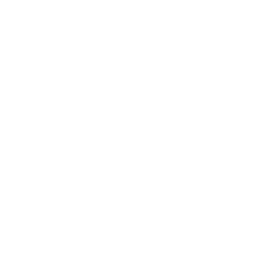
\includegraphics[width=8cm]{field.png}
    \caption{The displacement field preview as a user drags out the radius of a circular tine operation.}
\end{figure}

A full preview of the displacement field that would be applied with the current tool parameterization can also be rendered by pressing F.

\subsection{Script Editor}

Taking advantage of Javascript's dynamic nature, we provide the same object-oriented operation API built for our use to users. Scripts can be shared as URLs, enabling easy sharing of precise compositions. The editor's syntax highlighting is provided by the popular open source CodeMirror library.

\begin{figure}
    \includegraphics[width=8cm]{scripting.png}
    \caption{The script editor open above our application's main interaface. User's have access to all of the capabilities of the Javascript standard library as well as access to the marbling operation API.}
\end{figure}

\subsection{Limitations}

Although the rendering approach we used allows for arbitrary precision, it has expense proportional to ink-drop point density. As more drops are added, the rendering process slows significantly, and the user will notice a delay between releasing the mouse and seeing the results of their operation. A raster rendering approach, in which operations are applied to pixels and not points along ink-drop boundaries would enable GPU acceleration and frame rates sufficient to provide intra-operation animation.

Because of the single threaded nature of Javascript virtual machines, long rendering times impact UI responsiveness. Support for background threads is becoming more widespread, however it brings additional implementation complexity.

A fundamental limitation of this marbling approach is its simplicity. As opposed to more sophisticated fluid simulation approaches, it cannot reproduce highly dynamic behavior seen in some types of marbling.

\begin{figure}
    \includegraphics[width=8cm]{example1.png}
    \caption{A pattern created with a script that placed concentric circles, then ran circular tines emanating from the left and right of the canvas.}
\end{figure}

\begin{figure}
    \includegraphics[width=8cm]{example2.png}
    \caption{A mix of randomly placed drops and vortices.}
\end{figure}

\begin{figure}
    \includegraphics[width=8cm]{example3.png}
    \caption{Alternating horizontal and vertical tines create familiar floral patterns}
\end{figure}

\section{Conclusion and Future Work}

The provided tools enable a range of traditional marbling patterns, but they cannot easily express freeform tine patterns. Future work should explore enabling freehand operations. Lu and collaborators have recently published work extending the 2D marbling operations to 3D. An extension of this project may attempt to implement this work. 

\bibliography{references}
\bibliographystyle{plain}
\end{document}

